\begin{frame}[fragile]{\texttt{whoami}}
    
\pause

\begin{columns}

  \begin{column}{0.33\textwidth}
    \centering
    \begin{tikzpicture}
        \node[draw=white, line width=1pt, inner sep=0pt] {
            \includegraphics[width=\linewidth, angle=90]{media/phd-grad.jpg}
        };
    \end{tikzpicture}
    
    \captionof*{figure}{\shortstack{\footnotesize Recent Stanford PhD Graduate\\\textcolor{gray}{\scriptsize Used Julia throughout my research}}}
  \end{column}

  \pause

  \begin{column}{0.33\textwidth}
    \centering
    \begin{tikzpicture}
        \node[draw=white, line width=1pt, inner sep=0pt] {
            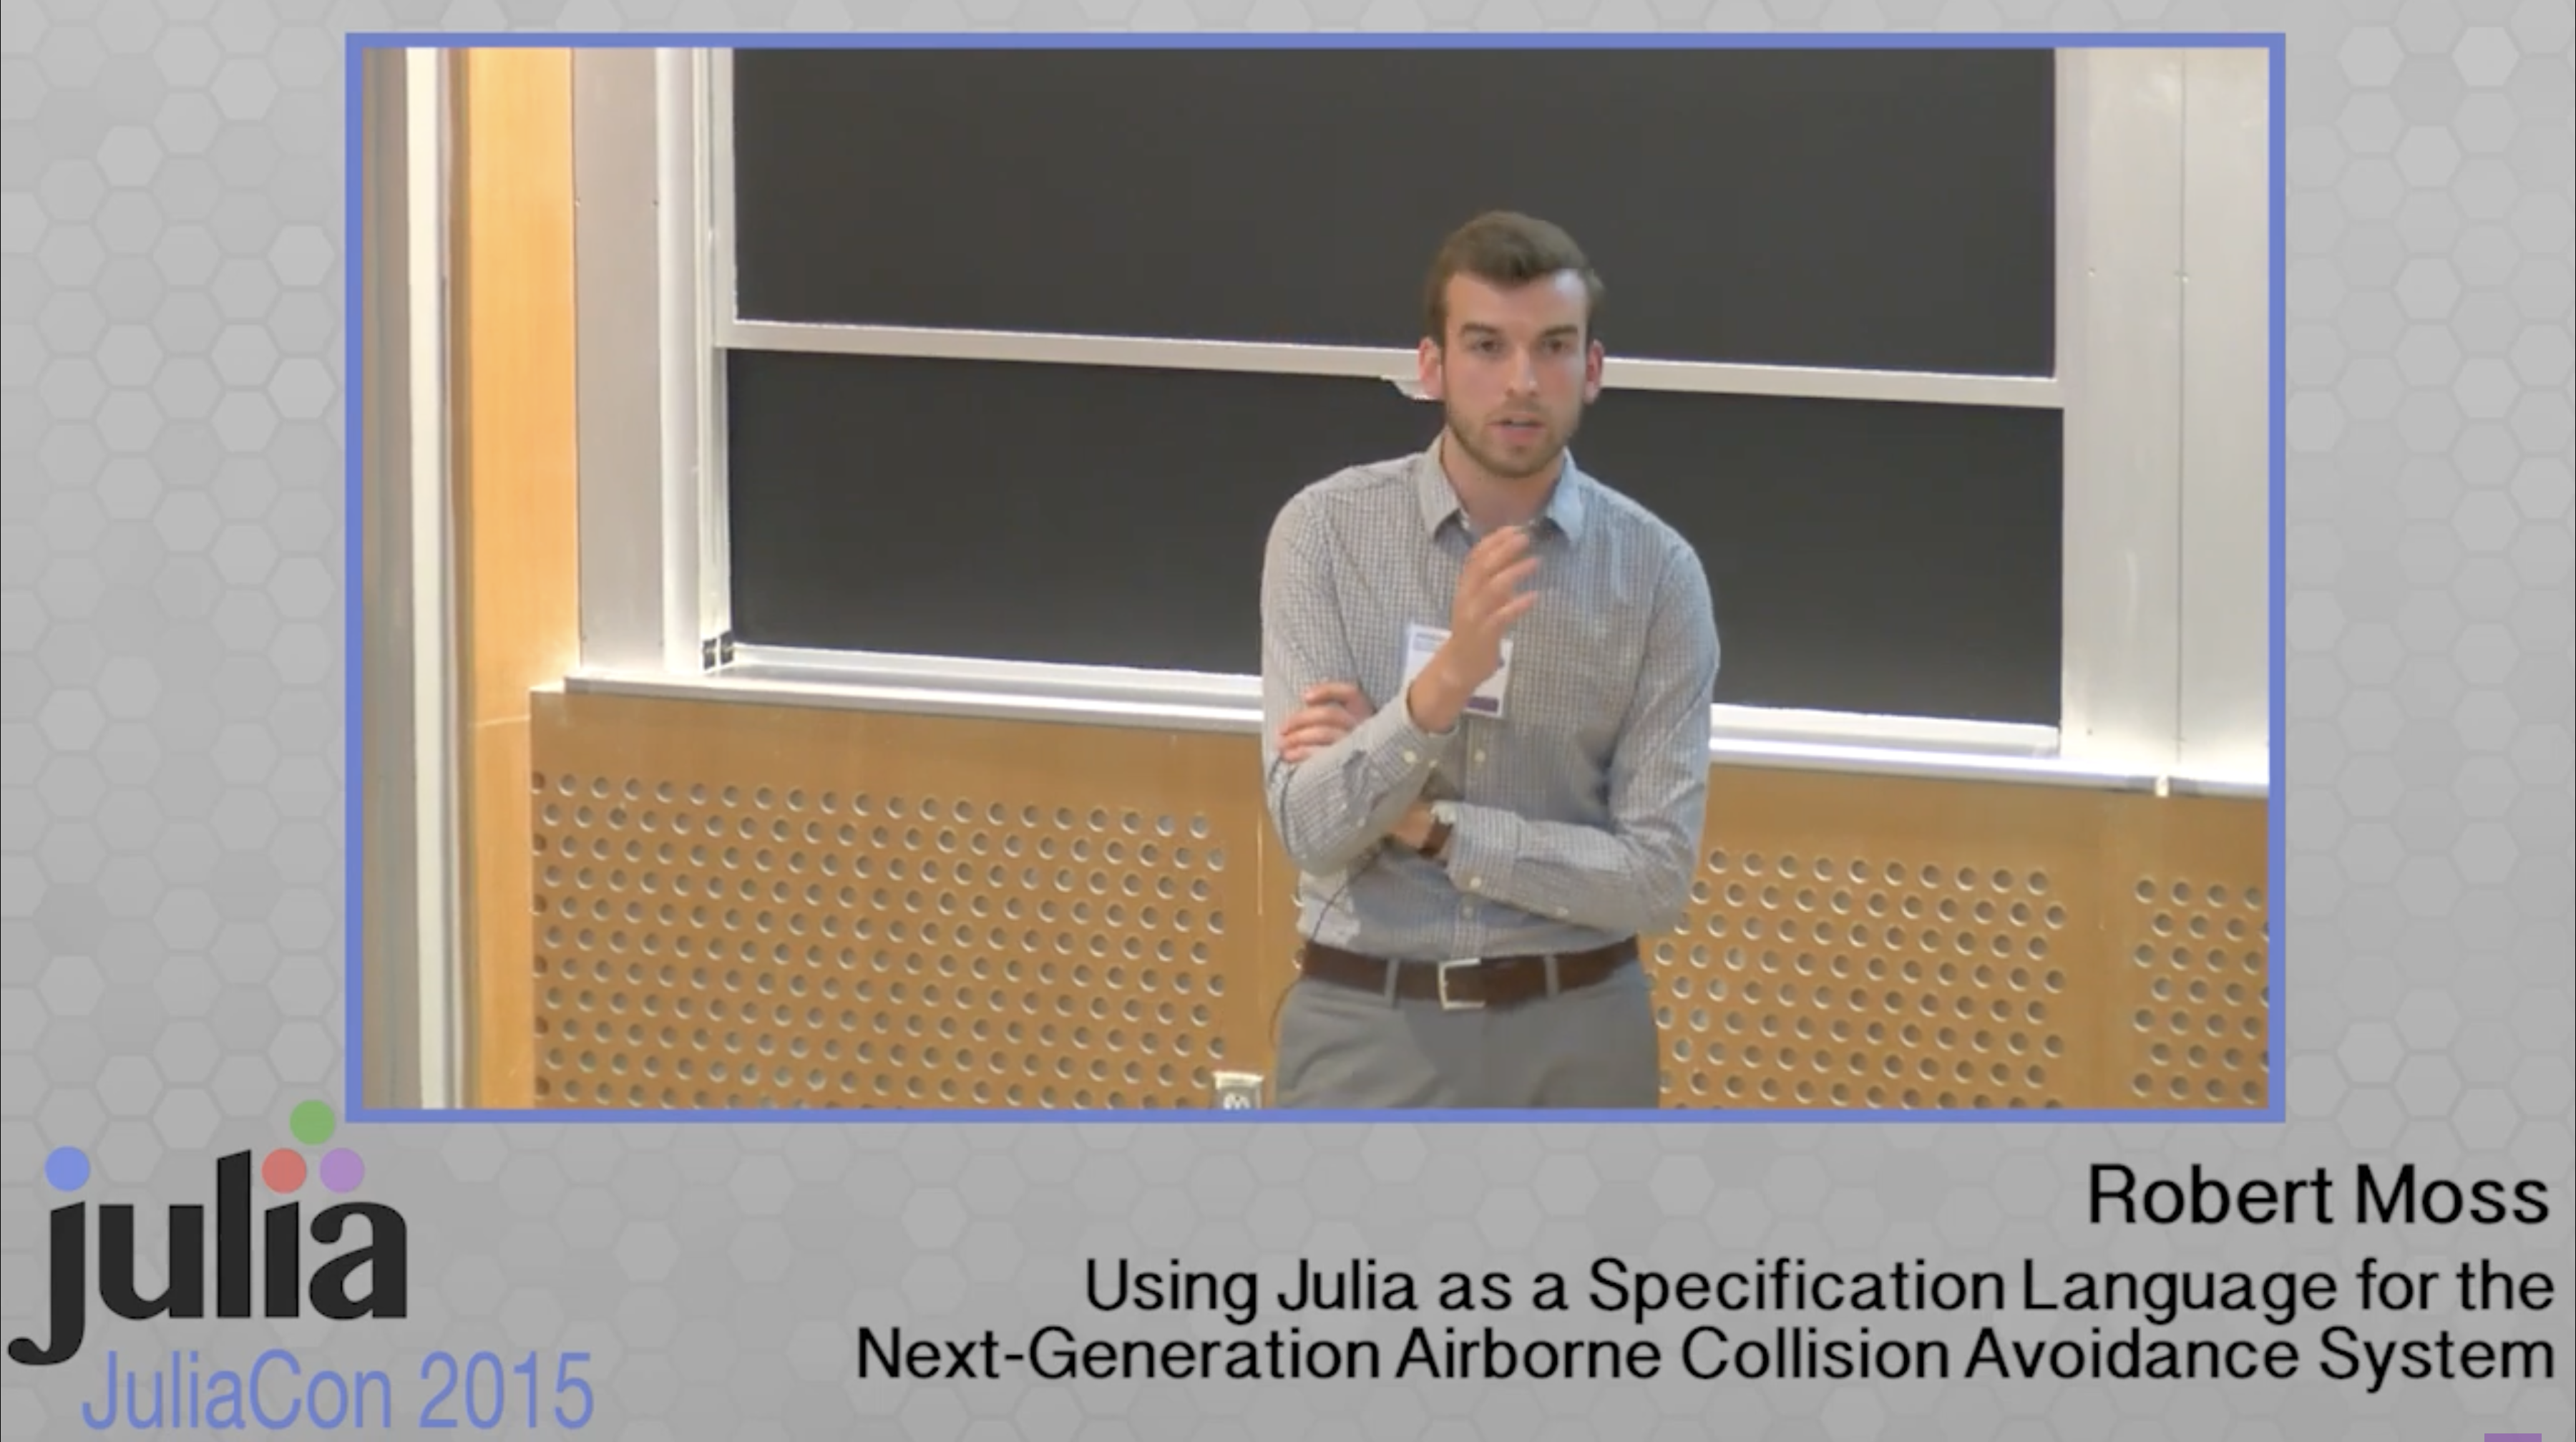
\includegraphics[width=\linewidth]{media/juliacon-2015.png}
        };
    \end{tikzpicture}

    \captionof*{figure}{\shortstack{\footnotesize Prev. at MIT Lincoln Laboratory\\\textcolor{gray}{\scriptsize Julia as a specification language}}}
  \end{column}

  \pause

  \begin{column}{0.33\textwidth}
    \centering
    
\includegraphics[width=\linewidth]{media/textbook-cover.png}
    
    \captionof*{figure}{\shortstack{\footnotesize Textbook Co-Author/Head TA\\\textcolor{gray}{\scriptsize Algorithms written in Julia}}}
  \end{column}

\end{columns}

\end{frame}